\section{Transformation to Polygonal Dual}
\label{sect:transformation-to-dual}

In this step of the pipeline, we take a filtered cluster graph \clustergraph{} and form a polygonal dual of thereof, resulting in the map \initmap{}.
To formalize the their relationship, we need the concept of the augmented dual:

\begin{definition}
The \emph{augmented dual} $G^+$ of a plane graph $G$ is the plane multigraph obtained by first placing a new vertex $v^+$ in the outer face of $G$, connecting it to all vertices on the outer face, in order, without introducing edge crossings, and then forming its dual.
\label{def:augmented-dual}
\end{definition}

\Cref{fig:transformation-augmented-dual} illustrates how the augmented dual $G^+$ of a plane graph $G$ (\cref{subfig:transformation-augmented-dual-1}) is formed.
We add the helper vertex $v^+$ and helper edges $\{v^+,\cdot\}$ in the outer face in \cref{subfig:transformation-augmented-dual-2}.
We draw the helper edges as in \cite{wagner2016algorithmen} because it does not matter where in the plane this helper vertex lies \emdash{} all that matters is that each pair of adjacent vertices on the outer face forms a new triangular face with $v^+$.
In \cref{subfig:transformation-augmented-dual-3}, we overlay the dual vertices and edges in red.
\Cref{subfig:transformation-augmented-dual-4} shows just the augmented dual of $G$.
%
\begin{figure}[H]
	\centering
	\subfigure[]{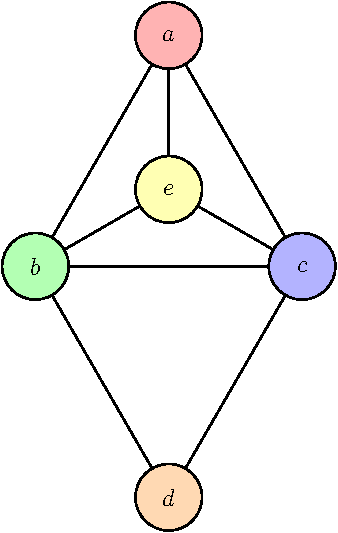
\includegraphics[height=130px]{Resources/Transformation-AugmentedDual-1.pdf}\label{subfig:transformation-augmented-dual-1}}
	\quad
	\subfigure[]{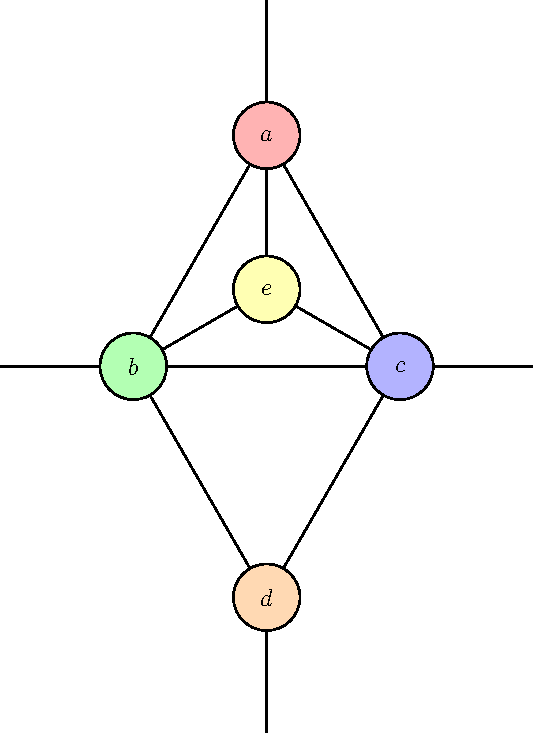
\includegraphics[height=130px]{Resources/Transformation-AugmentedDual-2.pdf}\label{subfig:transformation-augmented-dual-2}}
	\quad
	\subfigure[]{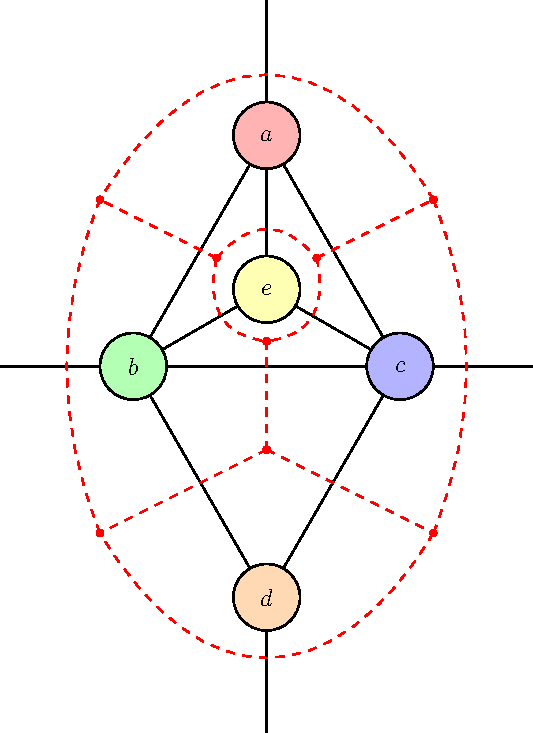
\includegraphics[height=130px]{Resources/Transformation-AugmentedDual-3.pdf}\label{subfig:transformation-augmented-dual-3}}
	\quad
	\subfigure[]{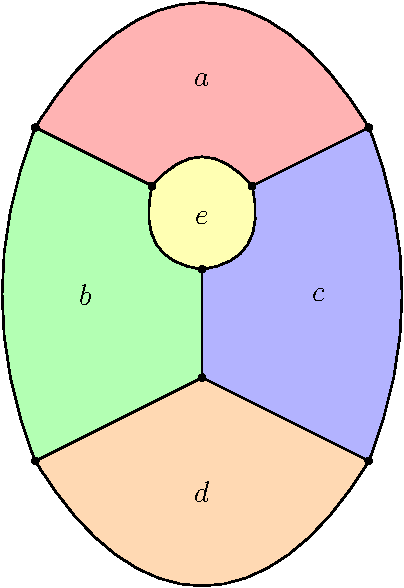
\includegraphics[height=130px]{Resources/Transformation-AugmentedDual-4.pdf}\label{subfig:transformation-augmented-dual-4}}
	\caption{Step-by-step representation of forming a plane graph's augmented dual.}
	\label{fig:transformation-augmented-dual}
\end{figure}

Note that analogous to the regular dual, the weak dual of the augmented dual of a plane graph $G$ is $G$ again, \ie{} $(G^+)^- = G$.

The augmented dual $G^+$ (\cref{subfig:transformation-augmented-dual-4}) of a biconnected and internally triangulated plane graph $G$ (\cref{subfig:transformation-augmented-dual-1}) essentially is a contact representation thereof.
In a polygonal dual, however, the edges cannot be curves and must be polylines instead.
The map \initmap{} can therefore be interpreted as a subdivision of the augmented dual $(\clustergraph{})^+$ in combination with a planar straight-line embedding thereof.



\paragraph{Algorithm Overview}

The underlying idea of creating the initial map \initmap{} is as follows:
Given a filtered cluster graph \clustergraph{}, we place vertices on edges of the outer face of \clustergraph{} (those edges bound additional triangular faces after adding the helper vertex in the process of forming the augmented dual) and inside the internal faces of \clustergraph{}.
We then connect these vertices if their corresponding faces are adjacent.
Connecting two vertices may require additional subdivision vertices or bends in order not to introduce edge crossings \emdash{} we use a single bend per edge.

In a preliminary step, we construct a planar straight-line drawing $\Gamma^\mathcal{C}$ of \clustergraph{}.
According to Fáry's theorem \cite{fary1948straight} \cite{wagner1936bemerkungen} \cite{stein1951convex}, such a drawing exists for every planar graph.
There are numerous popular algorithms to construct such an embedding such as Tutte's method \cite{tutte1963draw}, the shift method \cite{fraysseix1990draw}, or the Schnyder realizer method \cite{schnyder1990embedding}.



\clearpage
\paragraph{Algorithm Implementation}

\begin{algorithm}[H]
  \caption{Transformation to Polygonal Dual}
  \label{alg:transformation-to-dual}
  \SetKwData{Endpoints}{endpoints}
  \SetKwFunction{Appending}{appending}
  \SetArgSty{textrm}
  \vspace{5pt}
  \KwData{filtered cluster graph \clustergraph{} and a planar straight-line drawing $\Gamma^\mathcal{C}$ thereof}
  \KwResult{polygonal contract representation \initmap{} of \clustergraph{}, in the form of a 1-subdivision of the augmented dual of \clustergraph{} and planar straight-line drawing thereof}
  \vspace{10pt}
  create empty contact representation \initmap{}\;
  \ForEach{inner face $f$ in \clustergraph{}}{
    \label{line:transformation-loop1-start}
    add \quoted{inner face vertex} $v_f$ to \initmap{}\; \label{line:transformation-innerfacevertex}
    position $v_f$ at barycenter of $f$ in \clustergraph{} \label{line:transformation-barycenter1}\;
    \label{line:transformation-loop1-end}
  }
  \ForEach{edge $\{u,v\}$ in \clustergraph{}}{
    \label{line:transformation-loop2-start}
  	\If{$\{u,v\}$ is incident to two different internal faces $f, g$ in \clustergraph{} \label{line:transformation-incidentfacelookup1}}{
  	  add \quoted{subdivision vertex} $v_\text{sub}$ to \initmap{}\; \label{line:transformation-subdivisionvertex1}
  	  position $v_\text{sub}$ at midpoint of ${\{u,v\}}$ in \clustergraph{}\;
  	  add edge between $v_f$ and $v_\text{sub}$ to \initmap{}\;
  	  add edge between $v_\text{sub}$ and $v_g$ to \initmap{}\;
  	}
  	\ElseIf{$\{u,v\}$ is incident to a single internal face $f$ in \clustergraph{} \label{line:transformation-incidentfacelookup2}}{
  	  add \quoted{outer edge vertex} $v_{\{u,v\}}$ to $G_\text{init}$\; \label{line:transformation-outeredgevertex}
  	  position $v_{\{u,v\}}$ at midpoint of ${\{u,v\}}$ in \clustergraph{}\;
  	  add \quoted{subdivision vertex} $v_\text{sub}$ to \initmap{}\; \label{line:transformation-subdivisionvertex2}
  	  position $v_\text{sub}$ at midpoint of segment between barycenter of $f$ and midpoint of ${\{u,v\}}$ in \clustergraph{} \label{line:transformation-barycenter2}\;
  	  add edge between $v_{\{u,v\}}$ and $v_\text{sub}$ to \initmap{}\;
  	  add edge between $v_\text{sub}$ and $v_f$ to \initmap{}\;
  	}
  	\label{line:transformation-loop2-end}
  }
  \ForEach{incident edges $\{\{u,v\},\{v,w\}\}$ on outer face of \clustergraph{}}{
    \label{line:transformation-loop3-start}
    add \quoted{subdivision vertex} $v_\text{sub}$ to \initmap{}\; \label{line:transformation-subdivisionvertex3}
    position $v_\text{sub}$ at position of $v$ in \clustergraph{}\;
    add edge between $v_{\{u,v\}}$ and $v_\text{sub}$ to \initmap{}\;
    add edge between $v_\text{sub}$ and $v_{\{v,w\}}$ to \initmap{}\;
    \label{line:transformation-loop3-end}
  }
  \ForEach{vertex $u$ in \clustergraph{} \label{line:transformation-enumeratevertices}}{
    \label{line:transformation-loop4-start}
    $\Endpoints \gets ()$\;
    \ForEach{adjacent pair $(v,w)$ of neighbors of $u$ in counterclockwise order \label{line:transformation-enumerateedges}}{
      \If{$(u,v,w)$ bound a triangular face $f$ in counterclockwise order in \clustergraph{} \label{line:transformation-checktriangle}}{
        append $v_f$ to \Endpoints\;
      }
      \Else{
        append $v_{\{u,v\}}$ to \Endpoints\;
        append $v_{\{u,w\}}$ to \Endpoints\;
      }
    }
    \ForEach{adjacent pair $(v,w)$ in \Endpoints \label{line:transformation-insertsubdivisions}}{
      insert subdivision vertex connecting $v$ to $w$ between $v$ and $w$ in \Endpoints\;
    }
    define $f_u$ as internal face on \Endpoints in \initmap{}\;
    set weight of $f_u$ in \initmap{} to weight of $u$ in \clustergraph{}\;
    \label{line:transformation-loop4-end}
  }
  \Return \initmap{}
\end{algorithm}
\vfill



\paragraph{Algorithm Correctness}

To show the algorithm's correctness, we work with a helper graph, the \emph{augmented graph} $G_\text{aug}$, that can be obtained from $G_\text{emb}$ by adding a new helper vertex in the outer face of $G_\text{emb}$ and connecting it to all vertices on the outer face of $G_\text{emb}$, in order, without introducing edge crossings.
This is the same graph as used in the definition of the augmented dual in \cref{def:augmented-dual}.
Therefore $G_\text{aug}^* = G_\text{emb}^+$.

The polygonal dual of $G_\text{emb}$ produced by \cref{alg:transformation-to-dual} consists of five kinds of vertices: inner face vertices (\cref{line:transformation-innerfacevertex}), outer edge vertices (\cref{line:transformation-outeredgevertex}), subdivision vertices between two inner face vertices (\cref{line:transformation-subdivisionvertex1}), subdivision vertices between an inner face vertex and an outer edge vertex (\cref{line:transformation-subdivisionvertex2}), and subdivision vertices between two outer edge vertex (\cref{line:transformation-subdivisionvertex3}).
The inner face and outer edge vertices correspond to faces in the augmented graph and have degree 3, the subdivision vertices are essentially bends in the dual edges of the augmented graph and therefore have degree 2.
The following figure illustrates an example:
%
\begin{figure}[H]
	\centering
	\subfigure[]{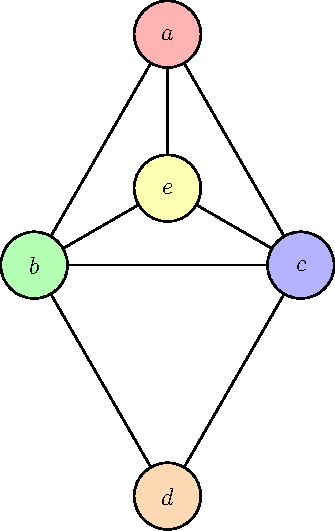
\includegraphics[height=70mm]{Resources/Transformation-Algorithm-Primal.pdf}\label{subfig:transformation-algorithm-primal}}
	\quad
	\subfigure[]{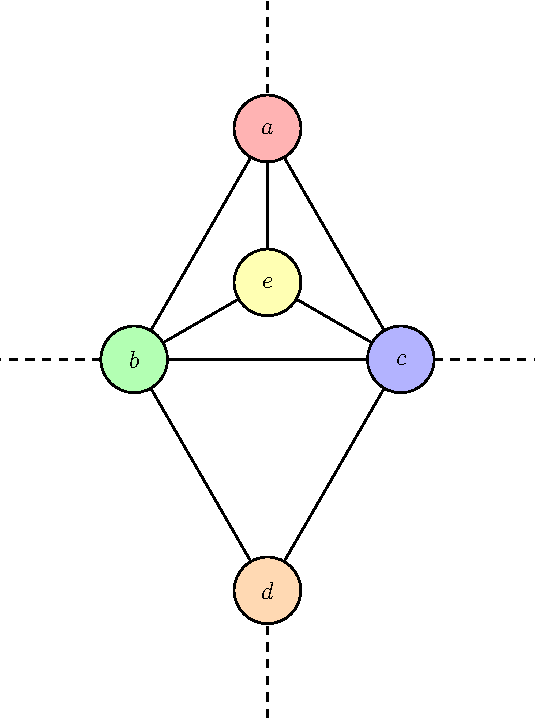
\includegraphics[height=70mm]{Resources/Transformation-Algorithm-Augmented.pdf}\label{subfig:transformation-algorithm-augmented}}
	\quad
	\subfigure[]{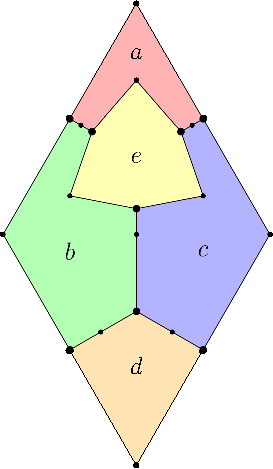
\includegraphics[height=70mm]{Resources/Transformation-Algorithm-Dual.pdf}\label{subfig:transformation-algorithm-dual}}
	\caption{An embedded cluster graph $G_\text{emb}$ (a), its augmented graph $G_\text{aug}$ (b), and its polygonal dual $G_\text{init}$ as produced by \cref{alg:transformation-to-dual} (c).}
	\label{fig:transformation-algorithm}
\end{figure}

Vertices in $G_\text{emb}^+$ are created for two following two scenarios:
%
\begin{itemize}
\item Every inner face $f$ of $G_\text{emb}$ induces a corresponding vertex $v_f$ in $G_\text{emb}^+$.
We create these vertices in \cref{line:transformation-innerfacevertex}.
\item Every outer edge $\{u,v\}$ of $G_\text{emb}$ forms an additional triangular face in $G_\text{aug}$ (one with the helper vertex) and therefore induces a corresponding vertex $v_{\{u,v\}}$ in $G_\text{emb}^+$.
We create these vertices in \cref{line:transformation-outeredgevertex}.
\end{itemize}

Every edge $\{u,v\}$ in $G_\text{emb}$ induces a dual edge in $G_\text{emb}^+$.
Let us go over the different kinds of edges we have and how we add them to $G_\text{emb}^+$ while guaranteeing the planarity of the embedding:
%
\begin{itemize}
\item Internal edges, \ie{} edges of $G_\text{emb}$ that do not lie on its outer face:
These edges are incident to two internal faces $f, g$ of $G_\text{emb}$.
Their dual edges in $G_\text{emb}^+$ therefore connect the vertices $v_f$ and $v_g$.
We draw these dual edges with a bend in \cref{line:transformation-subdivisionvertex1}.
\item Edges $\{u,v\}$ that lie on the outer face of $G_\text{emb}$:
These edges are incident to an internal face $f$ of $G_\text{emb}$ and a new triangular face with the helper vertex in $G_\text{aug}$.
In $G_\text{emb}^+$, their dual edges therefore connect the vertices $v_f$ and $v_{\{u,v\}}$.
We could draw these dual edges without a bend, but add a bend for consistency's sake in \cref{line:transformation-subdivisionvertex2}.
\item Helper edges $\{v,\cdot\}$ that are added to vertices $v$ on the outer face of $G_\text{emb}$ in $G_\text{aug}$:
These edges are incident to two new triangular faces in $G_\text{aug}$, namely the faces formed using $\{u,v\}$ and $\{v,w\}$, assuming $u$ and $w$ are the two neighbors of $v$ on the outer face of $G_\text{emb}$.
Their dual edges in $G_\text{emb}^+$ therefore connect the vertices $v_{\{u,v\}}$ and $v_{\{v,w\}}$.
We draw these dual edges with a bend in \cref{line:transformation-subdivisionvertex3}.
\end{itemize}

Due to our choice of bend locations, the generated embedding is planar:
We draw edges from the barycenter of all faces to the midpoints of their incident edges (in \crefrange{line:transformation-loop2-start}{line:transformation-loop2-end}); these edges cannot possibly cross.
The remainder of the edges (in \crefrange{line:transformation-loop3-start}{line:transformation-loop3-end}) partition the boundary of the outer face of $G_\text{emb}$.
Obviously, these two classes of edges do not cross and $G_\text{init}$ is therefore planar.

Once the algorithm has computed $G_\text{init}$, we construct an explicit representation of its faces.
We do so for $G_\text{emb}^+$ first (loop in \cref{line:transformation-enumerateedges}) and then insert the subdivision vertices (loop in \cref{line:transformation-insertsubdivisions}).
The face in $G_\text{emb}^+$ that corresponds to a vertex $v$ of $G_\text{emb}$ is bounded by vertices corresponding to internal faces of $G_\text{emb}$ that contain $v$, plus the vertices corresponding to the additional triangular faces in $G_\text{aug}$ in case $v$ lies on outer face of $G_\text{emb}$.
Iterating over adjacent pairs $(e_1, e_2)$ of incident edges in counterclockwise order correctly detects the internal faces between $e_1$ and $e_2$ and the case where $e_1$ and $e_2$ wrap around on the outside, in order.
The area sign check \cref{line:transformation-checktriangle} such that the wraparound case isn't misclassified as an internal face.
This would be the case for internal faces of $G_\text{emb}$ with two edges on the outer face, as is the case for vertex $v \coloneqq d$ and edges $e_1 \coloneqq \{d,b\}, e_2 \coloneqq \{d,c\}$ in \cref{fig:transformation-algorithm}.



\paragraph{Algorithm Runtime}

To compute the input graph's faces, we replace every edge with two inversely oriented, directed edges.
We then repeatedly pick any unmarked edge and form a directed cycle by following the next outgoing edge according to the embedding, marking the edges as we go.
Once all edges have been marked, we have found all faces.
The outer face is the one face whose interior is on the left when traveling along its bounding edges.
This can be implemented in $\bigTheta{\abs{V_\text{in}} + \abs{E_\text{in}}}$.

The input graph has $\bigTheta{\abs{V_\text{in}}}$ internal faces and they are all triangles, therefore we can compute their barycenter in $\bigTheta{1}$ each (\cref{line:transformation-barycenter1}, \cref{line:transformation-barycenter2}).
By keeping track of of which faces an edge of the input graph is incident to while computing the faces as outlined above, we allow for $\bigTheta{1}$ lookups in \cref{line:transformation-incidentfacelookup1} and \cref{line:transformation-incidentfacelookup2}.
The loop in \crefrange{line:transformation-loop1-start}{line:transformation-loop1-end} therefore runs in $\bigTheta{\abs{V_\text{in}}}$, the loop in \crefrange{line:transformation-loop2-start}{line:transformation-loop2-end} in $\bigTheta{\abs{E_\text{in}}}$, and the loop in \crefrange{line:transformation-loop3-start}{line:transformation-loop3-end} in $\bigTheta{\abs{E_\text{in}}}$.

The loop in \crefrange{line:transformation-loop4-start}{line:transformation-loop4-end} processes every vertex once in \cref{line:transformation-enumeratevertices} and and every edge twice \cref{line:transformation-enumerateedges}.
We can check if the vertices $u,v,w$ form a triangle in constant time (\cref{line:transformation-checktriangle}) by checking if there's an edge between $v$ and $w$.
Considering each of the $\bigTheta{\abs{V_\text{in}} + \abs{E_\text{in}}}$ vertices of the generated graph appears in \code{endpoints} in no more than two iterations of the loop in \crefrange{line:transformation-loop4-start}{line:transformation-loop4-end} and all those vertices have degree 3, we can find their shared neighbor in constant time and implement the entire loop to run in $\bigTheta{\abs{V_\text{in}} + \abs{E_\text{in}}}$.

%By keeping track of which faces in the generated graph correspond to which vertices in the source graph in \crefrange{line:transformation-loop4-start}{line:transformation-loop4-end}, the loop in \crefrange{line:transformation-loop5-start}{line:transformation-loop5-end} runs in $\bigTheta{\abs{V_\text{in}} + \abs{E_\text{in}}}$.

The entire algorithm can therefore be implemented to run in $\bigTheta{\abs{V_\text{in}} + \abs{E_\text{in}}}$.



\paragraph{Theoretical Bounds}

But do we have to subdivide edges of the augmented dual of our embedded cluster graph $G_\text{emb}$ in order to get a valid polygonal dual of $G_\text{emb}$?
Although the augmented dual $G_\text{emb}^+$ is plane by definition, it is not immediately obvious that there exists a planar straight-line embedding of $G_\text{emb}^+$ \emdash{} and that's what we need for it to be a polygonal contact representation.

In our case, however, $G_\text{emb}^+$ is simple, \ie{} there are no loops or multiple adjacencies.
Recall that $G_\text{emb}$ is 2-connected and internally triangulated.
Adding the helper vertex in the outer face of $G_\text{emb}$ and connecting it to all vertices on the outer face therefore creates a fully triangulated, simple graph.
In a simple triangulated graph, there are no two edges that are incident to the same faces (only those would create multiple adjacencies when forming the dual) and no edges that have the same face on both sides (only those would create loops when forming the dual) either.
The augmented dual $G_\text{emb}^+$ is therefore simple and, according to Fáry's theorem, there exists a planar straight-line embedding of $G_\text{emb}^+$ respecting its original combinatorial embedding and outer face.

In addition to having a planar straight-line embedding, $G_\text{emb}^+$ is also a cubic graph, \ie{} one in which all vertices have degree 3.
This is because $G_\text{emb}$ with the helper vertex is a triangulated graph, meaning every face is incident to exactly three edges, which turns into every vertex being incident to exactly three edges when forming the dual.
According to the results of Thomassen \cite{thomassen1992plane}, $G_\text{emb}^+$ is therefore area-universal.
This means that regardless of the concrete face weights that $G_\text{emb}$ prescribes, there exists a planar straight-line embedding of $G_\text{emb}^+$ realizing those weights/areas.

Even without subdividing edges in $G_\text{emb}^+$, we could therefore choose the initial map graph $G_\text{init}$ in such a way that it has perfect statistical accuracy already.
Such an embedding of $G_\text{emb}^+$ is non-trivial to compute though and creates undesired region shapes according to our other quality metrics.
Instead, we provide a very simple algorithm that subdivides all edges of the augmented dual once and leaves us with enough degrees of freedom to optimize for other quality metrics in \cref{sect:drawing-the-dual}.
